\section{Methodology and Experiment Setup}
\label{sec:methodology}
\subsection{Classifier Description}
Please give details of classifiers used in this project.

\subsection{Experiment Setup}

Fig. \ref{fig:infrastructure} shows the infrastructure of the whole system, which is divided into four parts: crawling module, parsing module, feature extracting module and sarcasm classifying module.

In the crawling module, we have developed a distributed crawling platform to collect a large-scale dataset from Twitter. The open-source tool Tweepy\cite{tweepy} was run on multiple machines in parallel, and all data will be centrally managed by the master node.

Raw tweets collected by the crawling module will be fed into the parsing module. The tool ark-twitter-nlp\cite{tweetnlp} was used to do tokenizing and POS tagging. After obtaining POS tagged tweets, TweeboParser\cite{kong2014dependency} will further run syntactic parsing which will generate syntactic dependency tree for each tweet. Named entity recognition was done by the tool in developed by Ritter et al\cite{Ritter11}\cite{Ritter12}. We applied sentiment analysis by utilizing the online machine learning framework Datumbox\cite{datumbox}. Due to the rate limit of this framework, we also created multiple parallel machine nodes to speed up sentiment analysis.

Parsed tweets are the input of the feature extracting module. We developed three feature extractors to extract corresponding features. After obtaining all tweet features, we are able to run the sarcasm classifying module, in which we used three classifiers, SVM with linear kernel, logitboosting with decision stump and bagging with SVM. 

\begin{figure}[htpb]
\centering
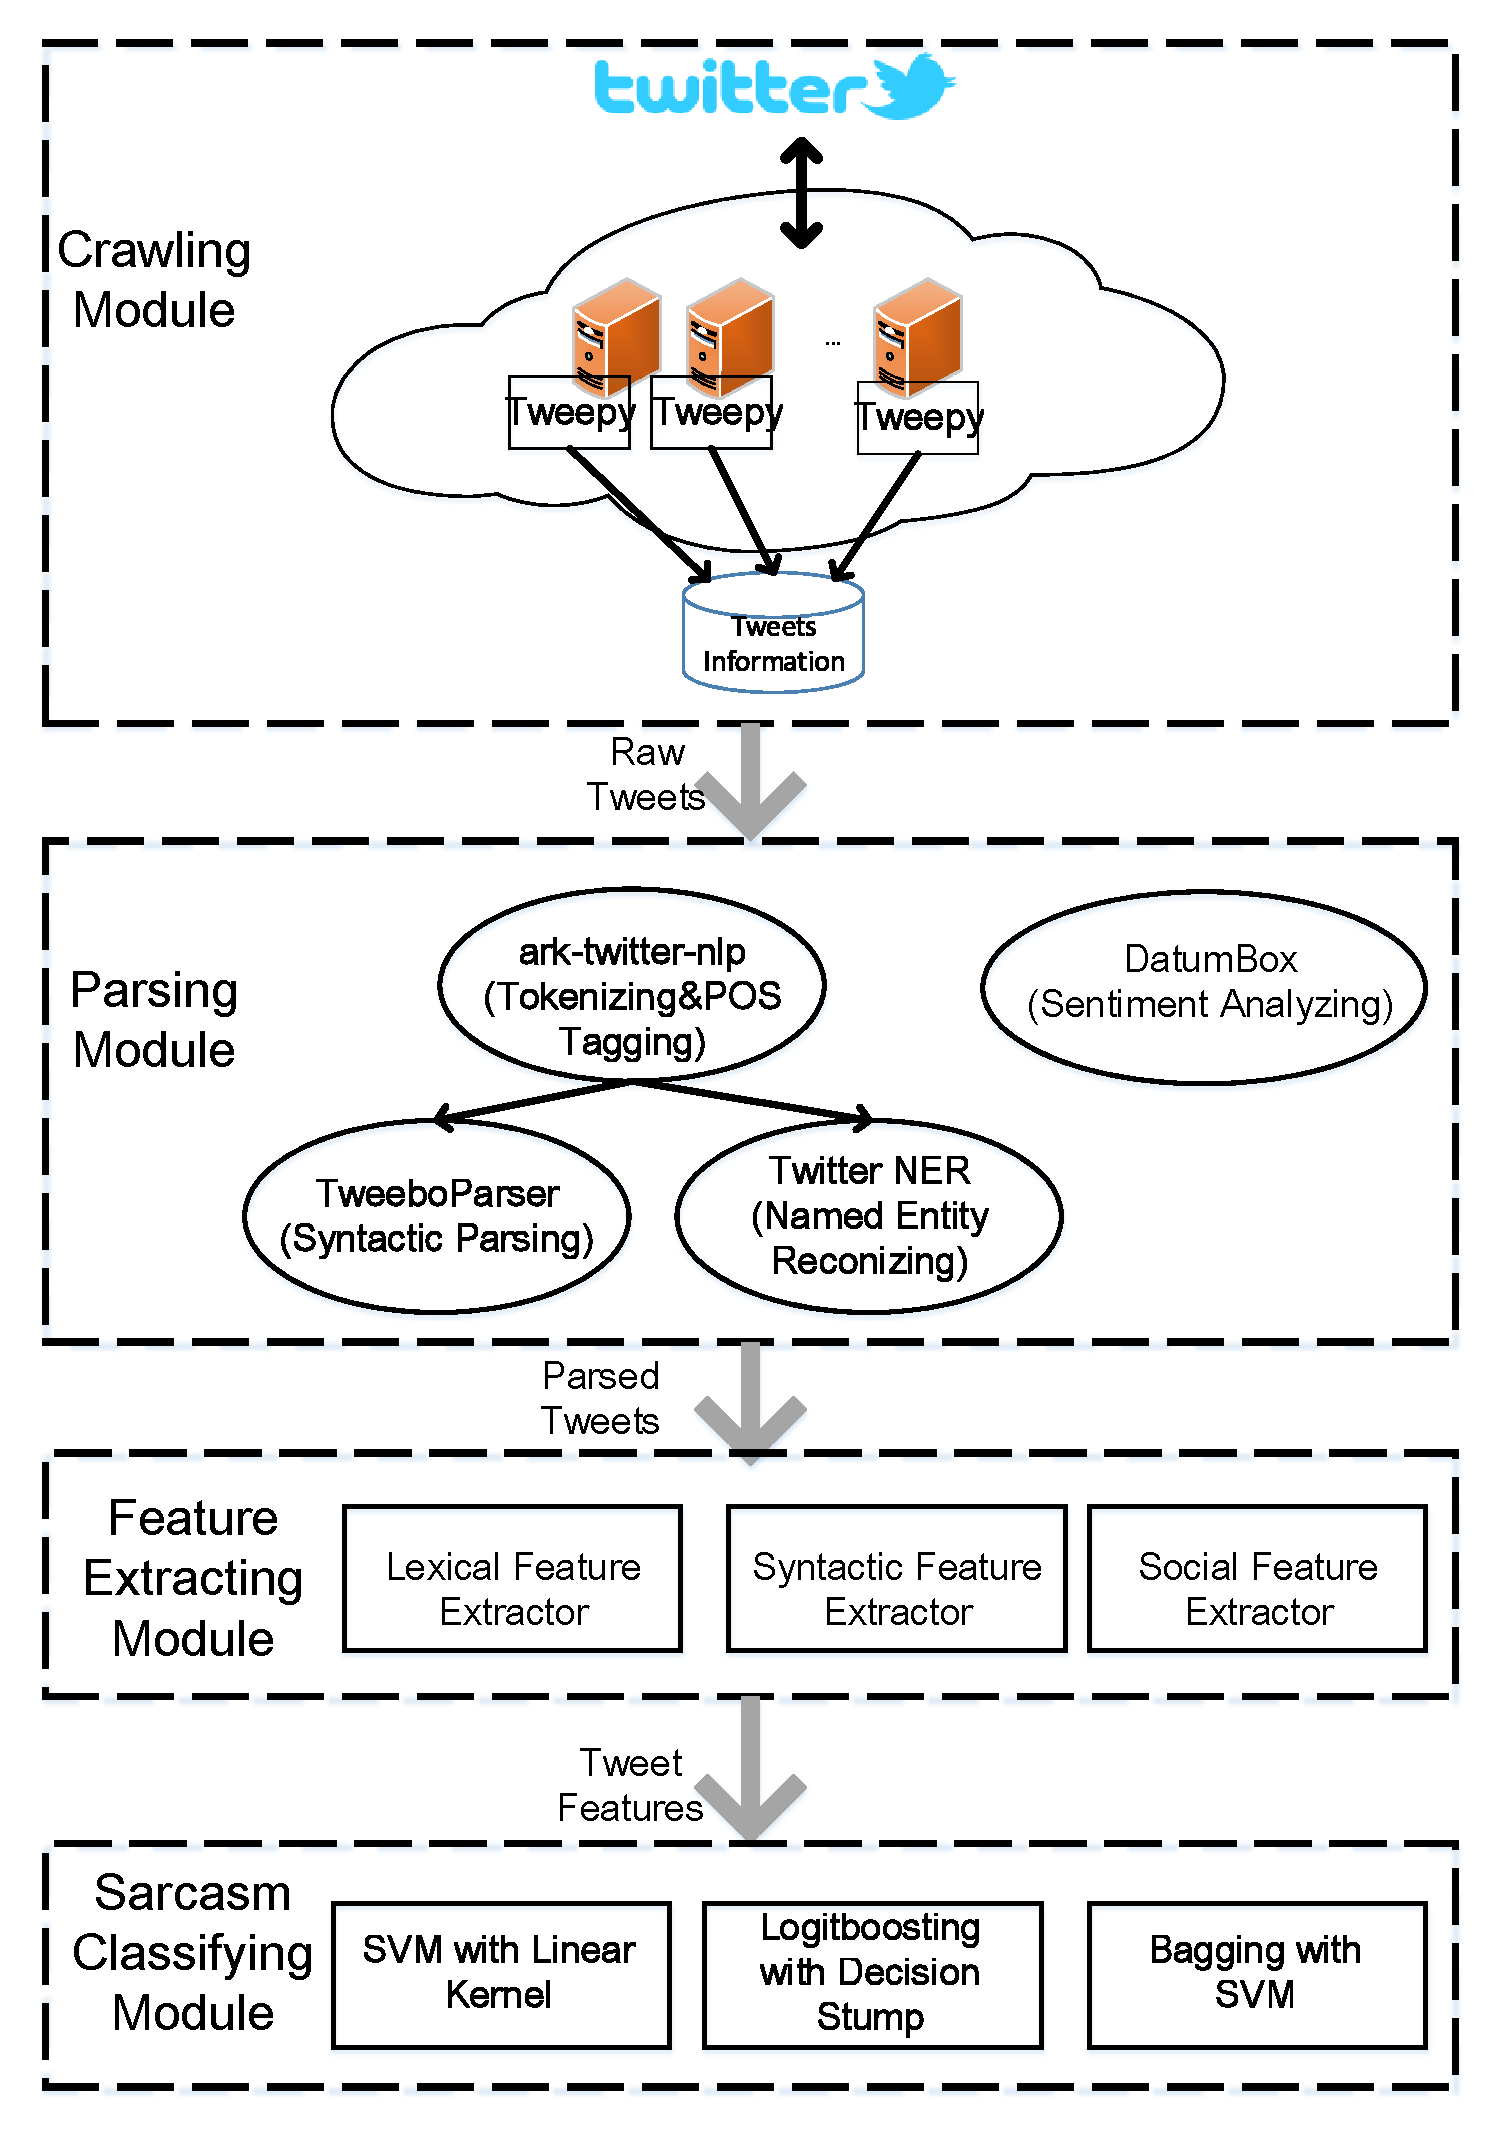
\includegraphics[scale=0.3]{infrastructure.eps}
\caption{The infrastructure of system setup.}
\label{fig:infrastructure}
\end{figure}
